% !TeX root = ../../main.tex

% Let $D$ be a compact subset of $\X$.
% Let $\dist(x, y) = \|x - y\|$ denote the distance between points $x,y\in D$ as a subspace of $\X$.
% For $A\subset D$ and $x\in D$ let
% \[\dist_A(x) = \min_{a\in A}\dist(x, a)\]
% denote the distance from $x$ to the set $A$.
% We will use open metric balls restricted to $D$ with the subspace topology
% \[\ball_\e(x) = \{y\in D\mid \dist(x, y) < \e\}\]
% and offsets
% \[A^\e = \{x\in D\mid \dist_A(x) < \e\}.\]

We now combine these results on the homology of surrounding pairs with information about both $\X$ as a metric space and our function.
We will then apply these results as a computable variation using Vietoris-Rips complexes that requires only pair-wise connectivity information.

Let $(\X,\dist)$ be a metric space and $D\subseteq \X$ be a compact subspace.
Let $f : D\to \R$ be a $c$-Lipschitz function and $B_\alpha = f^{-1}((-\infty, a])$ denote the $\alpha$-sublevel set of $f$ for $\alpha\in\R$.
We introduce a constant $\omega$ as a threshold that defines our ``boundary'' as a sub-levelset of the function $f$.
% In the next section we will explore both the challenges of computing, as well as the meaning, of the persistent homology of a function modulo the sub-levelset $B_\omega$.

Let $P$ be a finite subset of $D$ and $Q_\alpha := P\cap B_\alpha$ for $\alpha\in\R$.
Let $\zeta\geq\delta > 0 $ and $\omega\in \R$ be constants such that $P^\delta\subseteq D$.
Here, $\delta$ will serve as our communication radius where $\zeta$ is reserved for use in Section~\ref{sec:middle}.
  \footnote{We will set $\zeta = 2\delta$ in the proof of our interleaving with Rips complexes but the TCC holds for all $\zeta\geq\delta$.}
Unlike previous variations of the TCC~\ref{cavanna2017when} we do not require a change of scale in the geometric case.
Instead, we will enforce regularity close to the sub-levelset $B_\omega$ in terms of sub-levelsets $B_{\omega-c(\delta+\zeta)}$ and $B_{\omega+c(\delta+\zeta)}$.
Not only is this a more natural assumption, but it also allows us to replace the requirement that sensors detect the physical presence of a boundary with a threshold on the function values they observe.

\begin{lemma}\label{lem:psurj}
  Let $i : \hom_0(\cmp{\QQ^\of}, \cmp{P^\of})\to \hom_0(\cmp{\Q^\of}, \cmp{P^\delta})$.

  If $\B$ surrounds $D$ in $\X$ then $\dim~\hom_0(\cmp{\B}, \cmp{D})\geq \rk~i$.
\end{lemma}
\begin{proof}
  Choose a basis for $\im~i$ such that each basis element is represented by a point in $P^\of\setminus \QQ^\of$.
  Let $x\in P^\of\setminus \QQ^\of$ be such that $i[x] \neq 0$.
  So there exits some $p\in P$ such that $\dist(p, x) < \delta$ and $p\notin \QQ$, otherwise $x\in\QQ^\of$.
  Therefore, because $f$ is $c$-Lipschitz,
  \[ f(x)\geq f(p) - c\dist(x, p) > \fenn - c\of =\omega.\]

  So $x\in\cmp{\B}$ and, because $x\in P^\of\subseteq D$, $x\in D\setminus \B$.
  Because $i$ and $\ell : \hom_0(\cmp{\B}, \cmp{D})\to \hom_0(\cmp{\Q^\of}, \cmp{P^\of})$ are induced by inclusion $\ell[x] = i[x]\neq 0$ in $\hom_0(\cmp{\Q^\of}, \cmp{P^\of})$.
  That is, every element of $\im~i$ has a preimage in $\hom_0(\cmp{\B}, \cmp{D})$, so we may conclude that $\dim~\hom_0(\cmp{\B}, \cmp{D})\geq \rk~i$.
\end{proof}

Note that, while there is a surjective map from $\hom_0(\cmp{\B}, \cmp{D})$ to $\im~i$ this map is not necessarily induced by inclusion, as $\QQ^\of\not\subseteq \B$.
We therefore must introduce a larger space $B_{\omega+c(\delta+\zeta)}$ that contains $\QQ^\of$ in order to provide a criteria for the injectivity of $\ell : \hom_0(\cmp{\B}, \cmp{D})\to\hom_0(\cmp{\Q^\of}, \cmp{P^\of})$ in terms of $\rk~i$.

\[ \begin{tikzcd}
  (P^\of, \Q^\of) \arrow[hookrightarrow]{r}\arrow[hookrightarrow]{d} &
  (P^\of, \QQ^\of) \arrow[hookrightarrow]{d} \\
  %
  (D, \bb) \arrow[hookrightarrow]{r} &
  (D, B_{\omega+c(\delta+\zeta)}),
\end{tikzcd}\begin{tikzcd}
  (\cmp{B_{\omega+c(\delta+\zeta)}},\cmp{D})\arrow[hookrightarrow]{d}\arrow[hookrightarrow]{r} &
  (\cmp{\bb}, \cmp{D}) \arrow[hookrightarrow]{d}\\
  %
  (\cmp{\QQ^\of}, \cmp{P^\of}) \arrow[hookrightarrow]{r} &
  (\cmp{\Q^\of}, \cmp{P^\of}).
\end{tikzcd}\]

\begin{equation}\label{dgm:1}\begin{tikzcd}
  \hom_0(\cmp{B_{\omega+c(\delta+\zeta)}},\cmp{D})\arrow{d}{m} \arrow{r}{j} &
  \hom_0(\cmp{\bb}, \cmp{D}) \arrow{d}{\ell} \\
  %
  \hom_0(\cmp{\QQ^\of}, \cmp{P^\of}) \arrow{r}{i} &
  \hom_0(\cmp{\Q^\of}, \cmp{P^\of}).
\end{tikzcd}\end{equation}


\paragraph{Assumption 1}

% This is where we introduce our first assumption on the region surrounding $B_\omega$.
We will require the map $\hom_0(D\setminus B_{\omega+c(\delta+\zeta)}\hookrightarrow D\setminus B_\omega)$ to be \emph{surjective}---as we approach $\omega$ from \emph{above} no components \emph{appear}.
That is, in terms of $\omega$ as a super-levelset monotonically decreasing, no components \emph{apear} right \emph{before} $\omega$.
We note that, for a function in two dimensions, this translates to $1$-dimensional features disappearing right after $\omega$ in the sub-levelset filtration, as shown in Figure~\ref{fig:assumption1}.
% The reason for this dimension shift involves Alexander duality, and is discussed in more detail in Appendix~\ref{apx:duality} (see also~\cite{edelsbrunner12alexander}).
% That is, in terms of $\omega$ as a sub-levelset monotonically increasing, no components \emph{disappear} right \emph{after} $\omega$.

\begin{figure}[htbp]\label{fig:assumption1}
  \centering
  % 
\includegraphics[trim=50 190 0 200, clip, scale=0.2]{scripts/figures/scalar.png}
  % 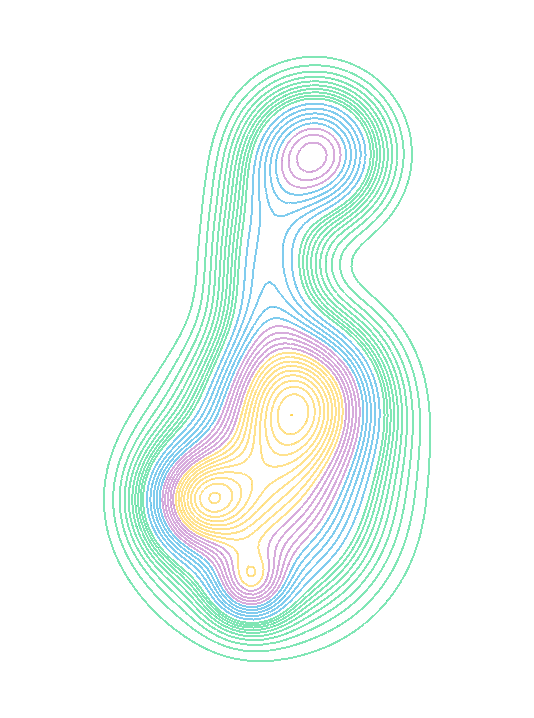
\includegraphics[trim=100 25 75 0, clip, angle=280, scale=0.25]{scripts/figures/scalar_contour.png}
  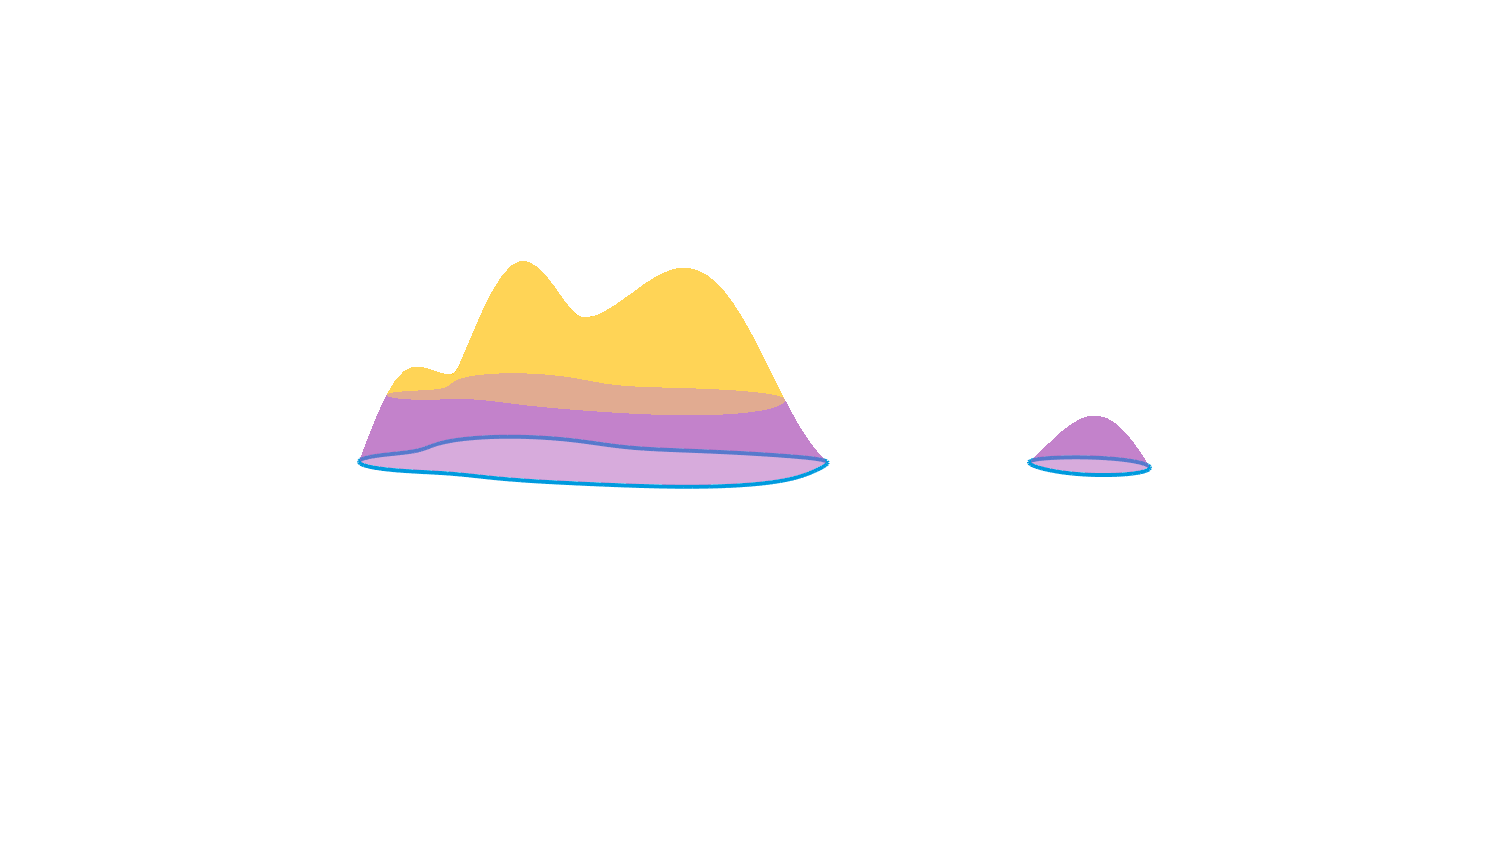
\includegraphics[trim=200 300 200 200, clip, width=0.5\textwidth]{scripts/figures/surf/ass1_C_side.png}
  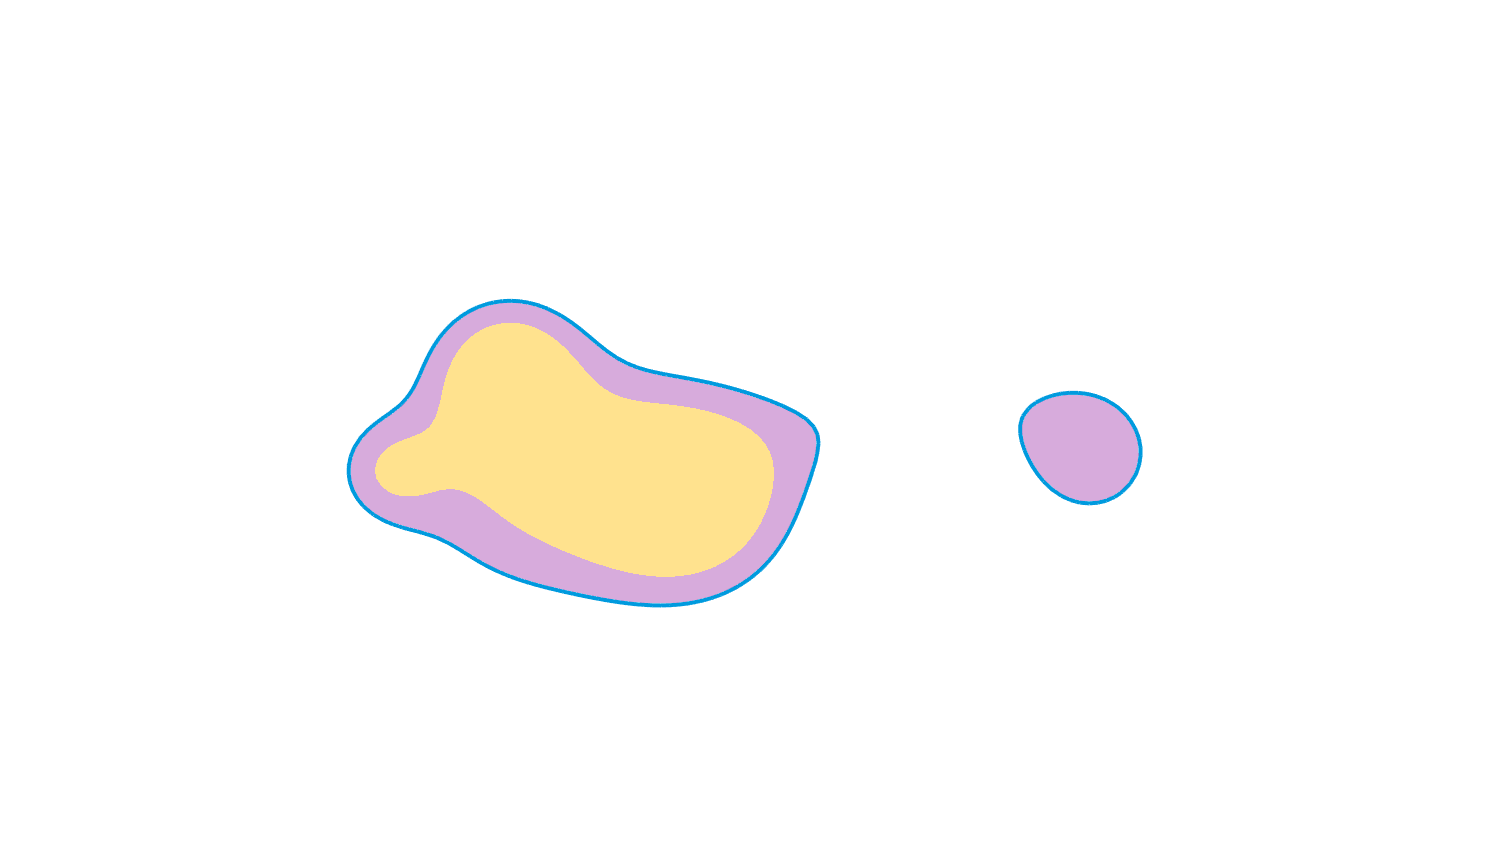
\includegraphics[trim=300 150 200 200, clip, width=0.3\textwidth]{scripts/figures/surf/ass1_C_top.png}
  
\includegraphics[trim=200 300 200 200, clip, width=0.5\textwidth]{scripts/figures/surf/ass1_D_side.png}
  
\includegraphics[trim=300 150 200 200, clip, width=0.3\textwidth]{scripts/figures/surf/ass1_D_top.png}
  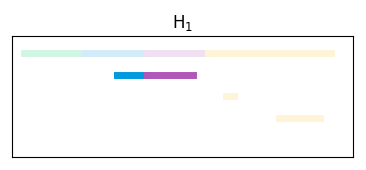
\includegraphics[scale=0.7]{scripts/figures/scalar_barcode_H1-masked.png}
  \caption{\textbf{(Assumption 1)} The blue levelset does not satisfy Assumption 1 as the smaller component is ``pinched out'' in the orange region.
            This can be seen in the barcode shown as a feature that dies in the purple region.}
\end{figure}

Now, the rank of the map $j$ is equal to the dimension of $\dim~\hom_0(\cmp{B_\omega}, \cmp{D})$ and our map $\ell$ induced by inclusion depends only on $\hom_0(\cmp{B_\omega}, \cmp{D})$ and $\im~i$.
The second assumption, which requires that nothing appears right \emph{before} $\omega$, will be used in Theorem~\ref{thm:algo_tcc} to provide a computable upper bound on $\rk~j$.

\begin{theorem}[Geometric TCC]\label{thm:geo_tcc}
  Let $D$ be a compact subset of $\X$ and $f : D\to\R$ be $c$-Lipschitz function.
  Let $\omega\in\R$, $\zeta\geq\of > 0$ be constants such that $\B$ surrounds $D$ in $\X$.
  Let $P\subset D$ be a finite collection of points and $Q_\alpha := P\cap B_\alpha$ for $\alpha\in\R$.
  Let $j : \hom_0(\cmp{B_{\omega+c(\delta+\zeta)}},\cmp{D})\to \hom_0(\cmp{\B},\cmp{D})$ and $i : \hom_0(\cmp{\QQ^\of}, \cmp{P^\of})\to \hom_0(\cmp{\Q^\of}, \cmp{P^\of})$ be induced by inclusion.

  If $j$ is surjective and $\rk~i\geq \rk~j$ then $D\setminus \B\subseteq P^\of$ and $\Q^\of$ surrounds $P^\of$ in $D$.
\end{theorem}
\begin{proof}
  Because $j$ is surjective by hypothesis $\rk~j = \dim~\hom_0(\cmp{\B},\cmp{D})$ so $\rk~j\geq \rk~i$ by Lemma~\ref{lem:psurj}.
  So $\rk~j = \rk~i$ with our assumption that $\rk~i\geq \rk~j$.
  Because $P$ is a finite point set we know that $\im~i$ is finite-dimensional and, because $\rk~i = \rk~j$, $\im~j=\hom_0(\cmp{\B}, \cmp{D})$ is finite dimensional as well.

  So $\im~j$ is isomorphic to $\im~i$ as a subspace of $\hom_0(\cmp{\Q^\of}, \cmp{P^\of})$ which, because $j$ is surjective, requires the map $\ell$ induced by inclusion to be injective.
  Therefore, $D\setminus\bb\subseteq P^\of$ and $\Q^\of$ surrounds $P^\of$ in $D$ by Lemma~\ref{lem:coverage}. %, Lemma~\ref{lem:cov_surrounds}.
\end{proof}
